% Document preamble
\documentclass[
12pt,
a4paper
]{article}

% Packages
%\usepackage[utf8]{inputenc}         % UTF-8 support
%\usepackage[T1]{fontenc}            % Proper hyphenation
\usepackage[romanian]{babel}        % Romanian characters support
\usepackage[top=9cm]{geometry}      % Increase top margin height
\usepackage{hyperref}               % Hyperlink support
\usepackage{graphicx}               % Image support

% Image configuration
\graphicspath{ {./src/} }

% Hyperlink configuration
\hypersetup{
colorlinks=true,
urlcolor=black,
}

% Page numbering
\pagenumbering{gobble} % uncomment if you want to disable it

% Custom commands
% Format: \newcommand{\command}{action (add '\ ' or '{}' if it won't add a space properly)}
\newcommand{\rom}[1]{\uppercase\expandafter{\romannumeral #1\relax}} % roman numerals

% Basic document info
\author{} % Empty author to not get a warn about missing author

\begin{document}
\begin{center}
 \vspace{9cm}
 {\LARGE Portofoliu}

 \vspace{0.5cm}
 {\Huge Limba și Literatura Română}

 \vspace{0.5cm}
 {\Large clasa a \rom{12}-a}

 \vspace{0.5cm}
 {2021-2022}

 \vspace{0.5cm}
 {\LARGE Dobrete Andrei-Robert}

 %\vspace{10.26cm}
 \vfill
 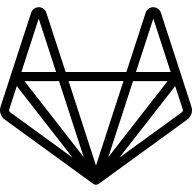
\includegraphics[height=\fontcharht\font`\B]{gitlab}
 \url{gitlab.com/Andy3153/eseuri_bac_romana}

 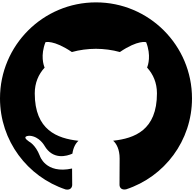
\includegraphics[height=\fontcharht\font`\B]{github}
 \url{github.com/Andy3153/eseuri_bac_romana}

 \vspace{0.5cm}
 {\large\LaTeX}
\end{center}
\end{document}
